\documentclass[twocolumn,10pt,a4j]{ltjsarticle}
\usepackage{kougai}

\title{娯楽ゲームの教育的活用を推進するWebサイトの開発}
\author{1732008 五十嵐美結  指導教員 須田 宇宙 准教授}
\date{}

\begin{document}

\maketitle

\section{はじめに}
%1章には,背景・問題点・目的を順番に書く.
%背景は,広く一般的な事柄を書いて,読む人に同意を抱かせつつ問題点につなぐ.
%問題点では,「〜という問題点がある」などのように,「問題」または「問題点」と言う単語を用いて,目的につなぐ.
%目的では,「そこで本研究では」から始めて,「〜を目的とする」で締める.
%以下は過去の卒業研究最終審査用の梗概の抜粋である.

%背景
近年,アクティブ・ラーニングとして授業活動にゲーミフィケーションといわれるゲームの娯楽性要素や,学習要素を盛り込んだシミュレーション等のゲーム(シリアスゲーム)を導入する動きが活発になってきている.
ゲーミフィケーションは楽しさ,目的意識,達成感の充実といったゲームの主要な要素を取り入れることによって授業への参加意欲や充実感の向上のために活用されている.
シリアスゲームはデジタルゲームの一種で主にコンピュータやタブレットなどを使用し,教育・医療・環境といった社会問題の解決を目的として,英語やプログラミング分野では実際に教育現場で活用されている.

%問題点
一方でデジタルゲームのうち、娯楽要素の多いゲームはゲーム依存症のイメージがあり、教育的なメリットは周知されておらず自宅での学習の妨げになる等の悪い印象が広まってしまっている。またこの問題のよって保護者からプレイの制限をされることで、ゲームから得られる学習機会の損失になるという問題点もある。
%また図\ref{fig:グラフ}のように子どもに悪い影響があるものとして保護者からの印象が悪く敬遠・制限されやすいことも問題である.



%Web版のシミュレータ教材は,オフライン状態で利用できないことが問題点として挙げられる.
%そこで,シミュレータ教材を電子書籍に搭載することで,オフライン状態でも利用できると考えた.
%しかし,搭載して動作させる上で,シミュレータ教材の機能が制限される場合がある.
%さらにシミュレータ教材をそのまま搭載しても,レイアウトの関係から利用しづらいという問題がある.
%この問題に対して,音響教育関係者がノウハウを共有し,お互いの開発したシミュレータ教材をカスタマイズして電子書籍化することが望ましいと考えている.

%目的
本研究では,学習を主目的としないデジタル娯楽ゲームの印象改善とそれらの持つ教育的効果の周知を図るために,様々な娯楽ゲームの持つ教育的なメリットをタグ付けしたWebサイトの開発をし,それにより印象が変化したかを保護者へのアンケート調査を行い評価することを目的とする.

%そこで本研究では,音響教育関係者が容易に電子教科書を制作できるよう,シミュレータ教材を搭載した電子教科書のサンプルの制作と,その開発ガイドラインを作成し公開することを目的とする.

%\vspace{1zh}
%\begin{figure}[h]
%\begin{center}
%\includegraphics[clip,width=90mm,height=50mm]{graph.pdf}
%\end{center}
%\caption{子どもへのゲームの影響について}
%\label{fig:グラフ}
%\end{figure}

\section{教育指向のゲームと娯楽ゲーム}
1章で紹介したシリアスゲームのようなゲームは学習に使用するために開発されたゲームなので教育効果が分かりやすく,保護者や教育者が導入し易くなっている。一方で娯楽ゲームはあくまで娯楽が主目的に開発されたゲームで,それから得られる教育効果が明示されているわけではない.そのため推奨されにくく,また依存症・ゲーム脳等のイメージが広まっていることから悪い影響があると思われプレイ制限に繋がってしまう.



%\section{エンターテイメントゲームについて}
%2章では,研究テーマとして取り上げた内容(この例では「電子教科書」についての研究だった)について説明する.その他,数式を用いて理論を説明することも可能である.

%本稿でのデジタルエンターテイメントゲームは家庭用ゲーム機やパソコン,タブレット,スマートフォン等でプレイするコンピュータゲームを指し、カテゴリはアクションやRPG,アドベンチャーなど多岐にわたる.シリアスゲームに挙げられるシミュレーションゲームも含まれるが,ここでは学習を目的としない娯楽指向のゲームについて示す.


\section{研究内容}
研究内容としてはWebサイトを作成し小中学生対象の娯楽ゲームの記事を載せたものを小中学生の子を持つ保護者に見てもらう.記事には後尾楽ゲームの持つ教育的なメリットについて記述し,

研究成果としては以下の通りである。
\begin{itemize}
\item 12個のゲームの記事をWebサイト上で公開
\item サイト閲覧後アンケート
\item アンケート内に見る前についての項目
\end{itemize}

アンケート \url{https://docs.google.com/forms/d/e/1FAIpQLSeZEQzh9D3b3QD1fZ9-Qtdazw49zxFw_te0srnpZdiXSZy4Lg/viewform}

%\section{Webサイト制作と評価方法}
%掲載するエンターテイメントゲームは様々な種類のものを用意し,それぞれのゲームの種類やプレイによって得られるだろう教育的メリットでジャンル分けしタグ付けを行う.タグは,創造性,協調性,社会理解,デジタル理解,自然理解などの他,ワード検索もできるようにする予定である.またタグの他に,授業の教科に関連付けを行い教科からも検索できるようにする.図\ref{fig:スクショ}のゲームの詳細ページを示す.①の部分は検索機能でタグやキーワードから検索ができる欄である.②の部分はゲームのスクリーンショットとゲームプレイによって得ることが期待される教育的メリットについての詳細や具体例を記述する.

%評価にはアンケート調査で行う.対象者は小中学生の子を持つ保護者で,マーク形式で作成し,最後に自由記述欄を設ける.
\vspace{1zh}
\begin{figure}[h]
\begin{center}
 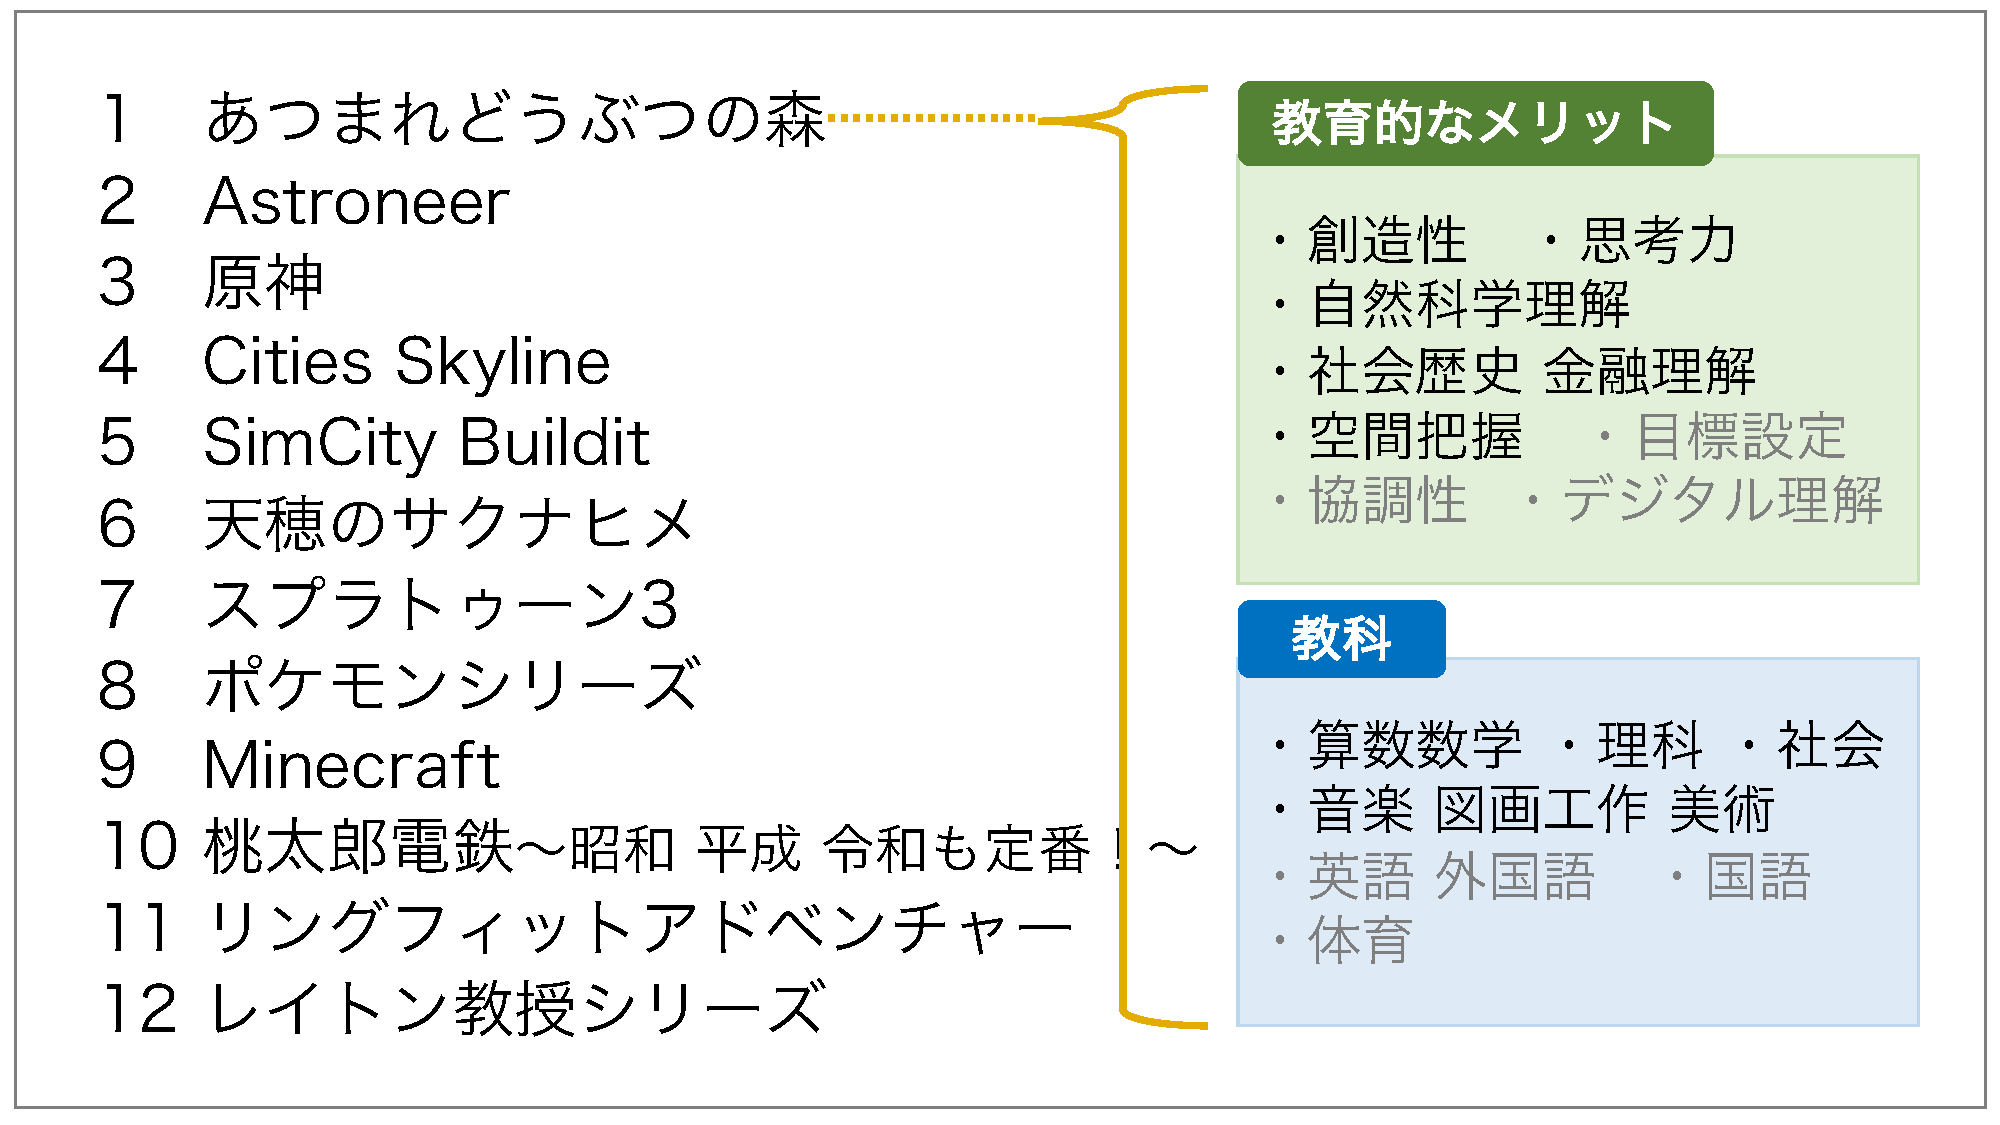
\includegraphics[clip,width=95mm,height=55mm]{games.pdf}
\end{center}
 \caption{ゲーム一覧とタグ例}
 \label{fig:スクショ}
\end{figure}

%3章には,最終審査用の梗概では,やったことを示す.
%コンテンツを作成した場合にはコンテンツのスクリーンショットなどを用いる.
%調査が主であれば,調査の概要と結果のグラフなどを使用する.

%この文章では1章が長すぎるので,見た目のバランスが悪い.
%通常の梗概の割合は左側に1章と2章,右側に3章と4章のように並ぶ.
%もちろん多少の前後は有るので,きっちりと合わせなくても良い.

%通常,図は2枚程度である.
%図1枚+表1面でも構わない.
%梗概を書き始める前に,使用する図を決めてからレイアウトしていくと雰囲気がつかみやすくて良い.


\section{おわりに}


%\section{今後の予定}
%今後は,ゲームの種類と情報の収集とWebサイトの作成,また評価に用いるアンケートの作成をGoogle Formsにて行う予定である.アンケート調査の対象者の募集も同時に行う.
%中間審査用の梗概では4章のタイトルとして「今後の予定」,最終審査用の梗概では「おわりに」などを用いる.
%たいてい2〜3行程度でまとめる.

\begin{thebibliography}{99}
\bibitem{gameanq} ASMARQ : ``ゲームと子どもに関するアンケート調査'', \url{https://www.asmarq.co.jp/data/mr201409game/}, 2022/8/19参照
\bibitem{tvgame} 坂元 章 : ``21世紀はテレビゲーミング社会 ―娯楽主導から有効利用ヘ―'', 特定非営利活動法人日本シミュレーション&ゲーミング学会, 2000年 10 巻 1 号 p.4-13, 2000.
\end{thebibliography}

\end{document}
